% !TeX root = main.tex
\section{Comparing airfoils}

We compare the following airfoils (as asked in the question)

\begin{itemize}
    \item Selig \textbf{S1223} high lift low Reynolds number airfoil
    \item Eppler \textbf{E220} low Reynolds number airfoil
    \item Martin Hepperle \textbf{MH45} for flying wings
\end{itemize}

These data files (coordinates) are available on the \href{https://m-selig.ae.illinois.edu/ads/coord_database.html}{UIUC airfoil database}. The profiles are shown in figure \ref{fig:q2-diff-airfoils}.

\begin{figure}[ht]
    \centering
    \begin{subfigure}[b]{0.3\textwidth}
        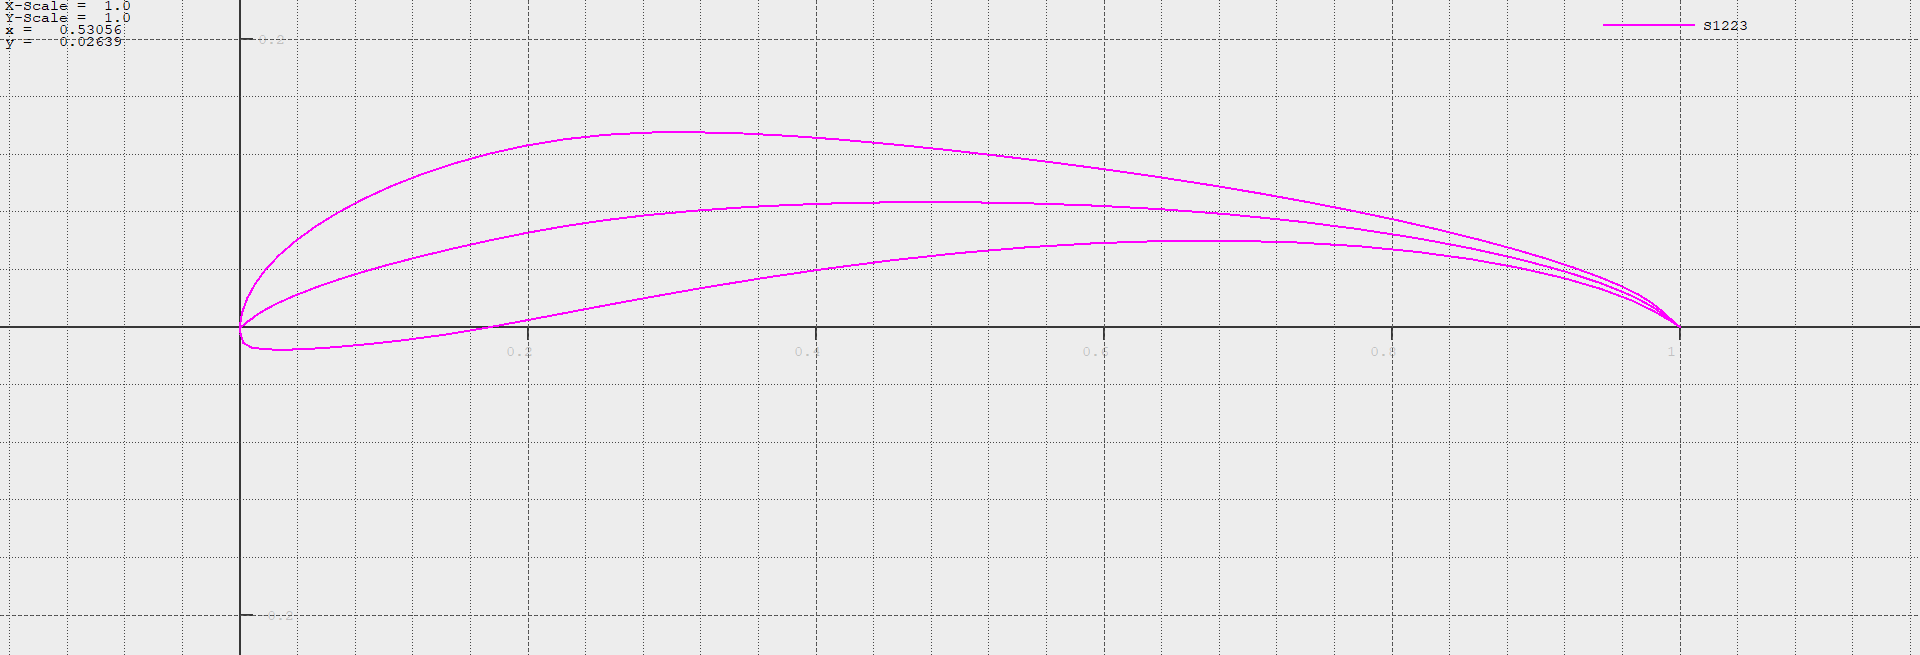
\includegraphics[width=\textwidth]{s1223-prof.png}
        \caption{S1223}
    \end{subfigure}
    \begin{subfigure}[b]{0.3\textwidth}
        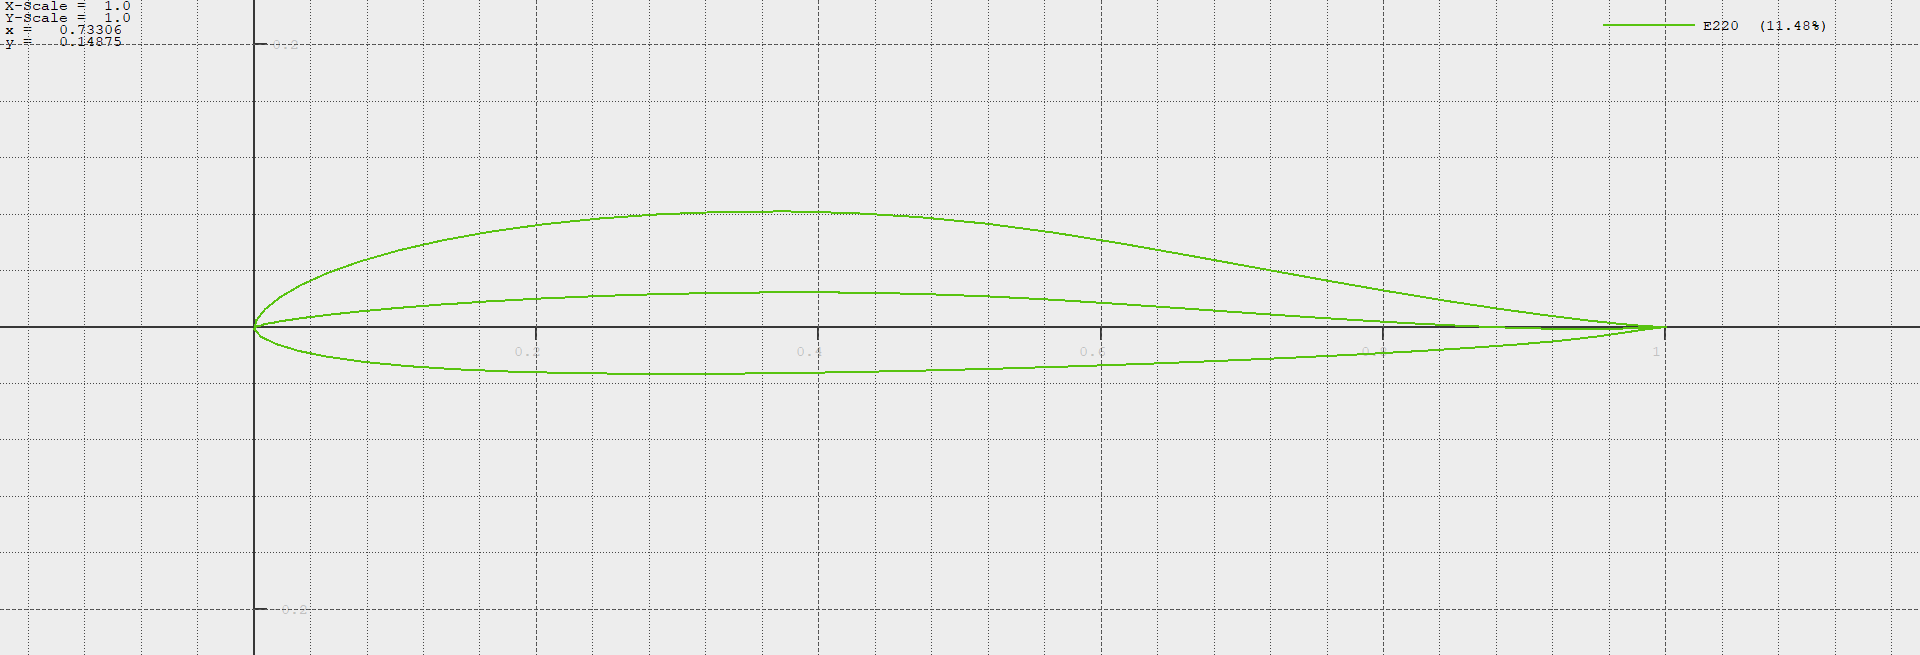
\includegraphics[width=\textwidth]{e220-prof.png}
        \caption{E220}
    \end{subfigure}
    \begin{subfigure}[b]{0.3\textwidth}
        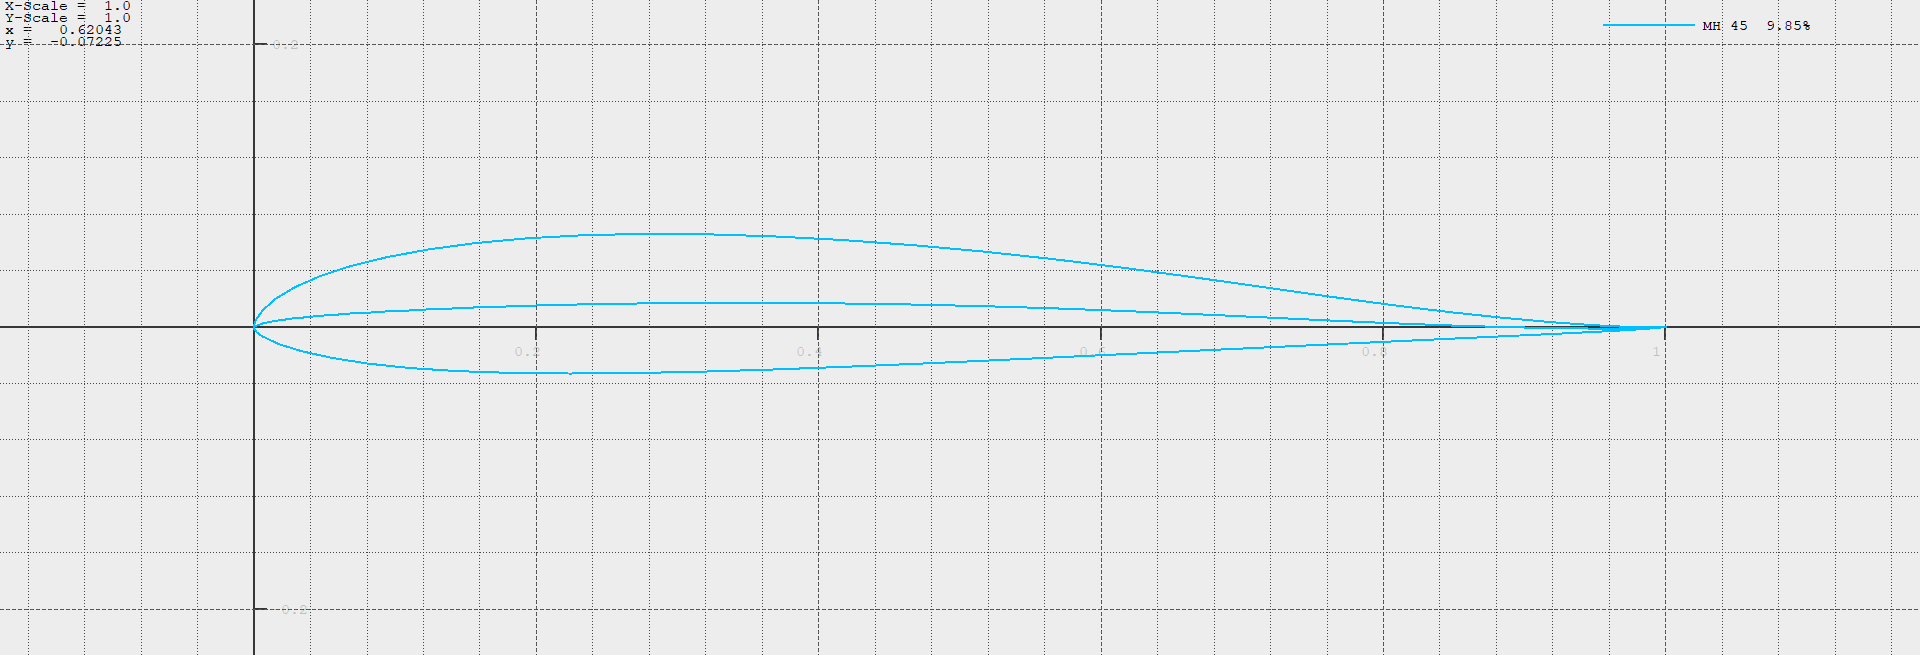
\includegraphics[width=\textwidth]{mh45-prof.png}
        \caption{MH45}
    \end{subfigure}
    \caption{Different airfoils}
    \label{fig:q2-diff-airfoils}
    \small
        All profiles as visible in \texttt{Direct Foil Design} of XFLR.
\end{figure}

\subsection{S1223}

The Selig \textbf{S1223} has a high positive camber in the middle. This will give it superior lift (compared to other two). The results can be seen in figure \ref{fig:s1223-analysis}.

\begin{figure}[ht]
    \centering
    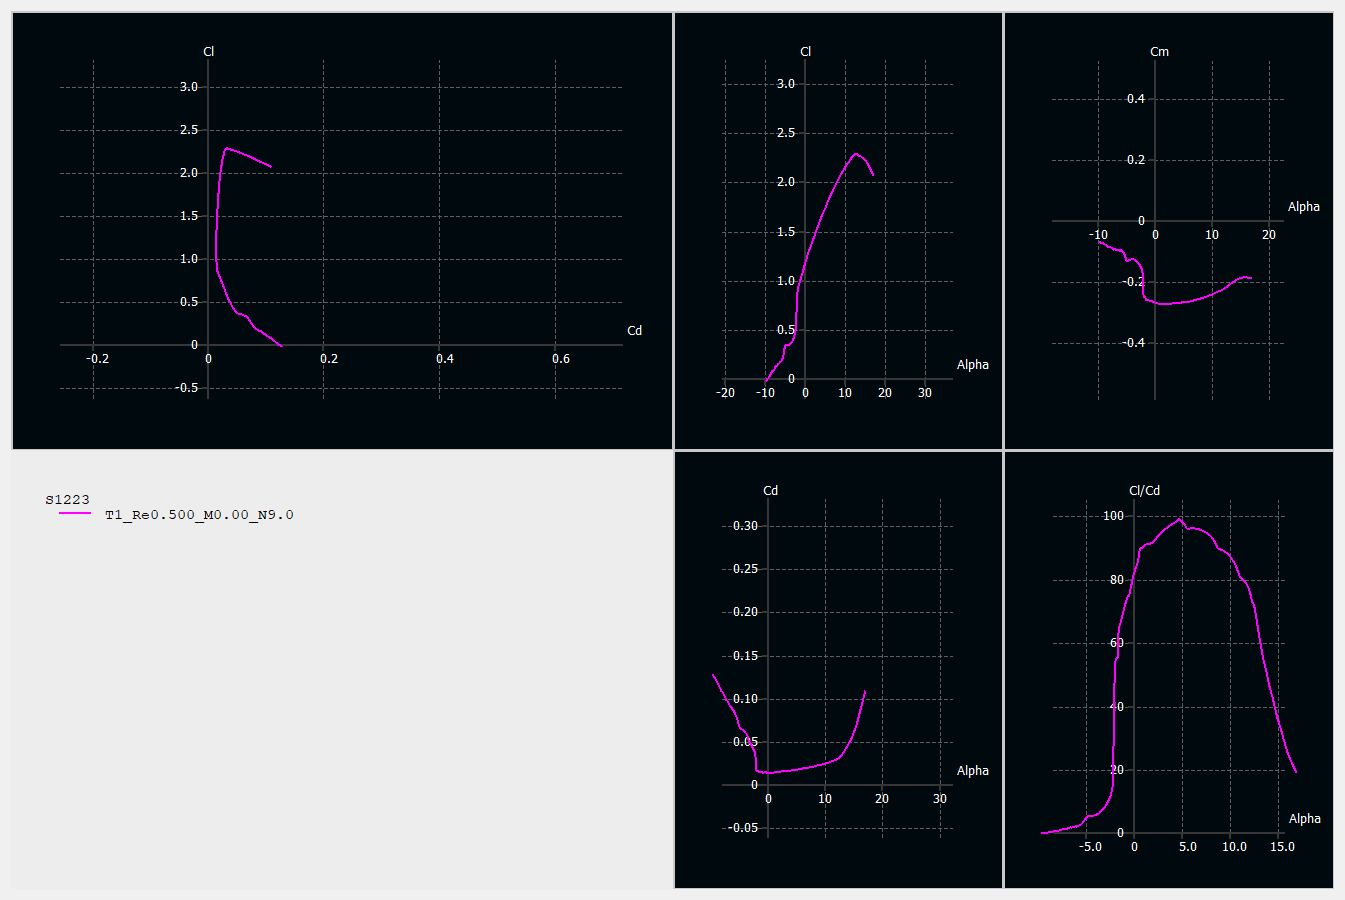
\includegraphics[width=\textwidth]{s1223-analysis.png}
    \caption{XFLR Analysis of S1223 Airfoil}
    \label{fig:s1223-analysis}
\end{figure}

\paragraph{For $C_l$}
The maximum $C_l$ occurs at $\alpha=12.6^\circ$.

\paragraph{For $\sfrac{C_l}{C_d}$}
The maximum $\sfrac{C_l}{C_d}$ occurs at $\alpha = 4.7^\circ$.

\paragraph{For $C_m$}
The $C_m$ graph follows a linear path for most of the positive $\alpha$ (small angles). It reaches the peak (most favorable) at $\alpha = 15.8^\circ$.

\subsection{E220}

The Eppler \textbf{E220} has a lower camber than S1223. It has much lesser moment, but the lift is lower. The results can be seen in figure \ref{fig:e220-analysis}.

\begin{figure}[ht]
    \centering
    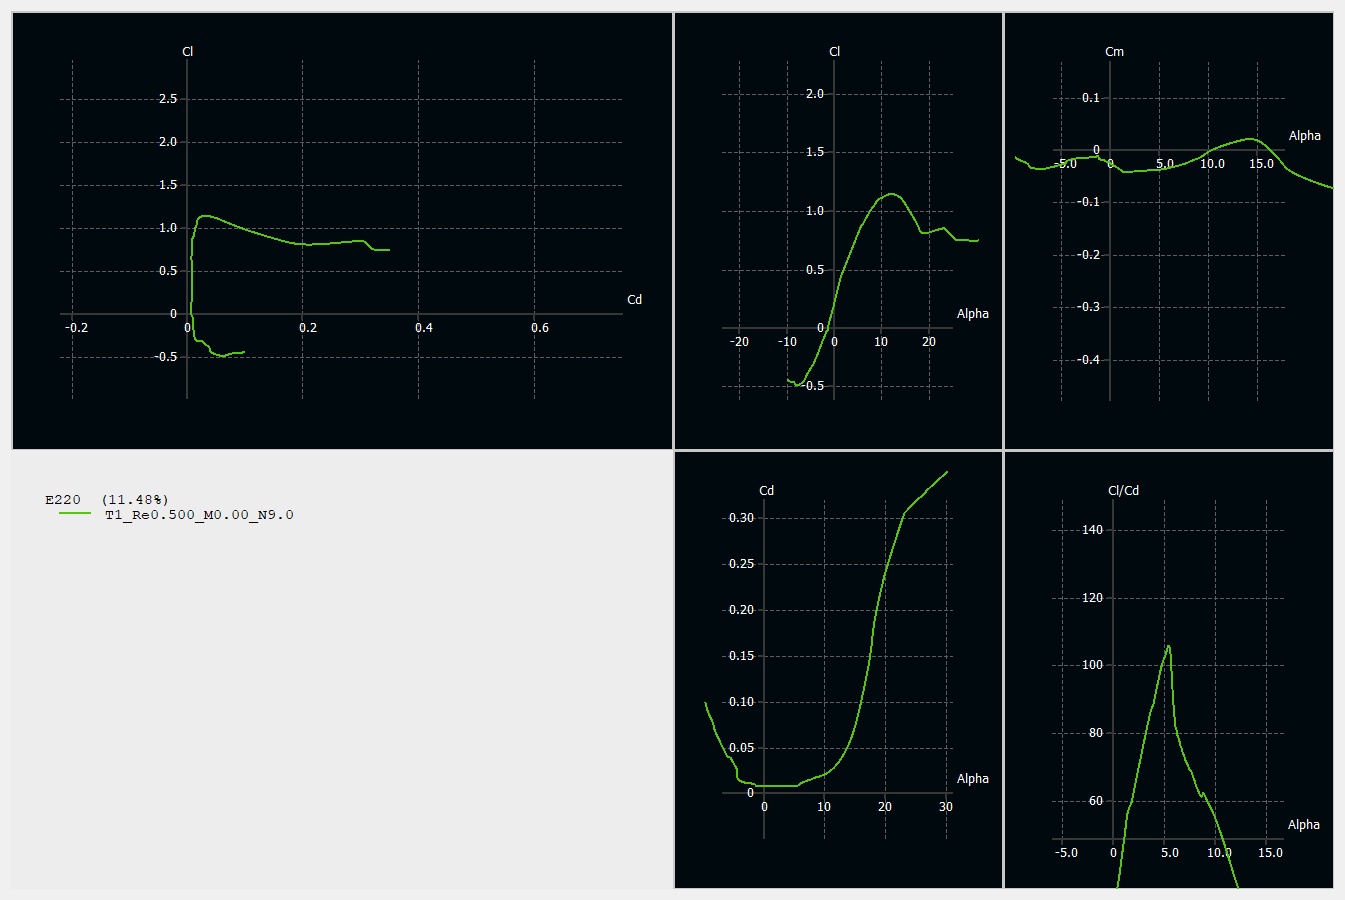
\includegraphics[width=\textwidth]{e220-analysis.png}
    \caption{XFLR Analysis of E220 Airfoil}
    \label{fig:e220-analysis}
\end{figure}

\paragraph{For $C_l$}
The maximum $C_l$ occurs at $\alpha=12.1^\circ$.

\paragraph{For $\sfrac{C_l}{C_d}$}
The maximum $\sfrac{C_l}{C_d}$ occurs at $\alpha = 5.4^\circ$.

\paragraph{For $C_m$}
The $C_m$ graph follows a linear path for most of the positive $\alpha$ (small angles). It reaches approximately zero at $\alpha = 10.3^\circ$.

\subsection{MH45}
Martin Hepperle \textbf{MH45} has a low camber (like E220). It has better lift and moment curves. The results can be seen in figure \ref{fig:mh45-analysis}.

\begin{figure}[ht]
    \centering
    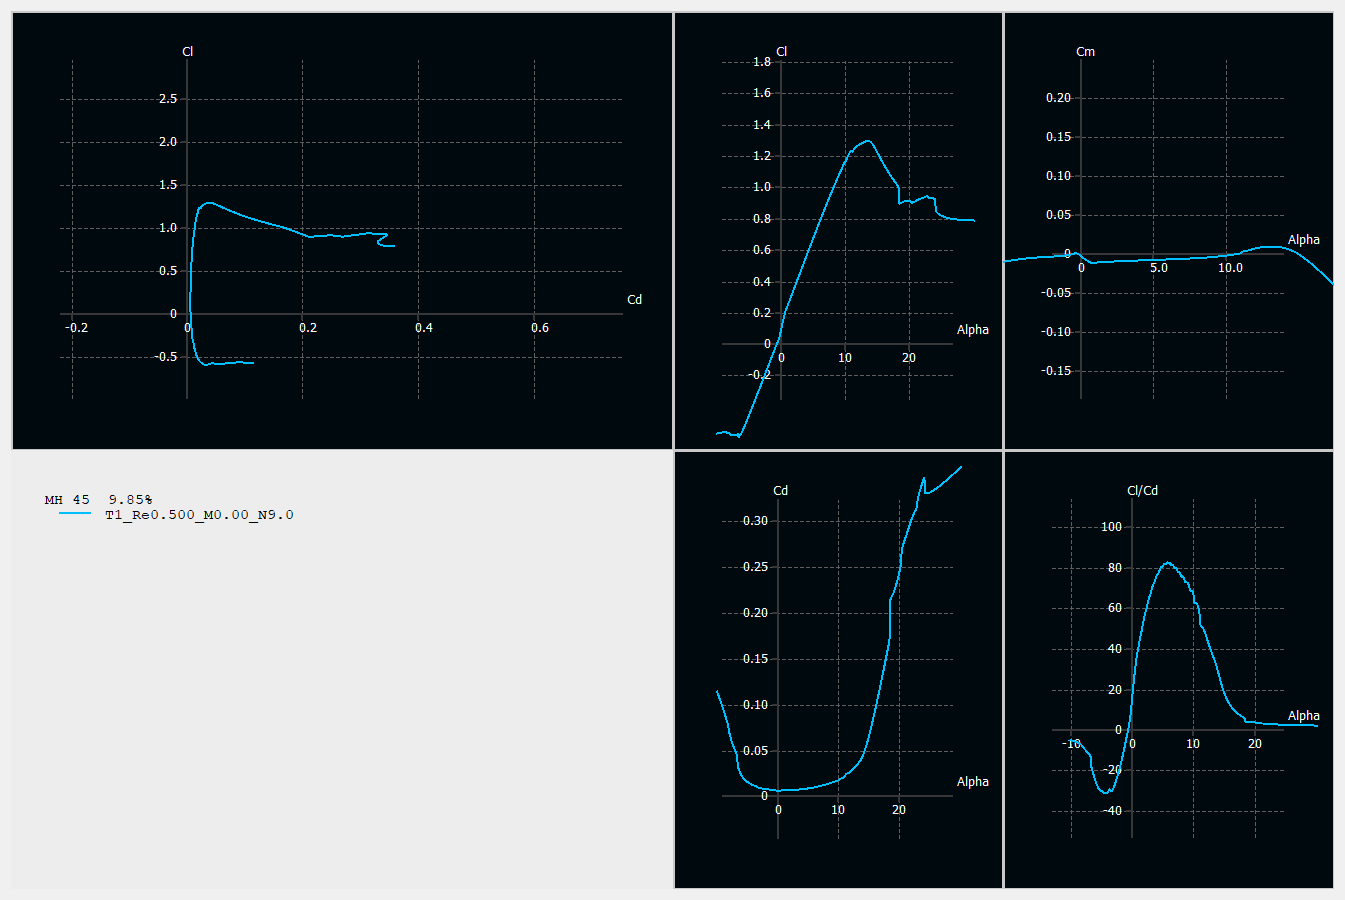
\includegraphics[width=\textwidth]{mh45-analysis.png}
    \caption{XFLR Analysis of MH45 Airfoil}
    \label{fig:mh45-analysis}
\end{figure}

\paragraph{For $C_l$}
The maximum $C_l$ occurs at $\alpha=13.6^\circ$.

\paragraph{For $\sfrac{C_l}{C_d}$}
The maximum $\sfrac{C_l}{C_d}$ occurs at $\alpha = 5.8^\circ$.

\paragraph{For $C_m$}
The $C_m$ graph follows a linear path for most of the positive $\alpha$ (small angles). It is very close to zero. A plane designed using this airfoil might not even need a tail (only change center of gravity a little and have big ailerons). It is near zero at $\alpha = 10.7^\circ$.

\subsection*{Summary}

A summary of the performance of all airfoils is shown in figure \ref{fig:q2-af-comp}

\begin{figure}[ht]
    \centering
    \begin{subfigure}[b]{0.45\textwidth}
        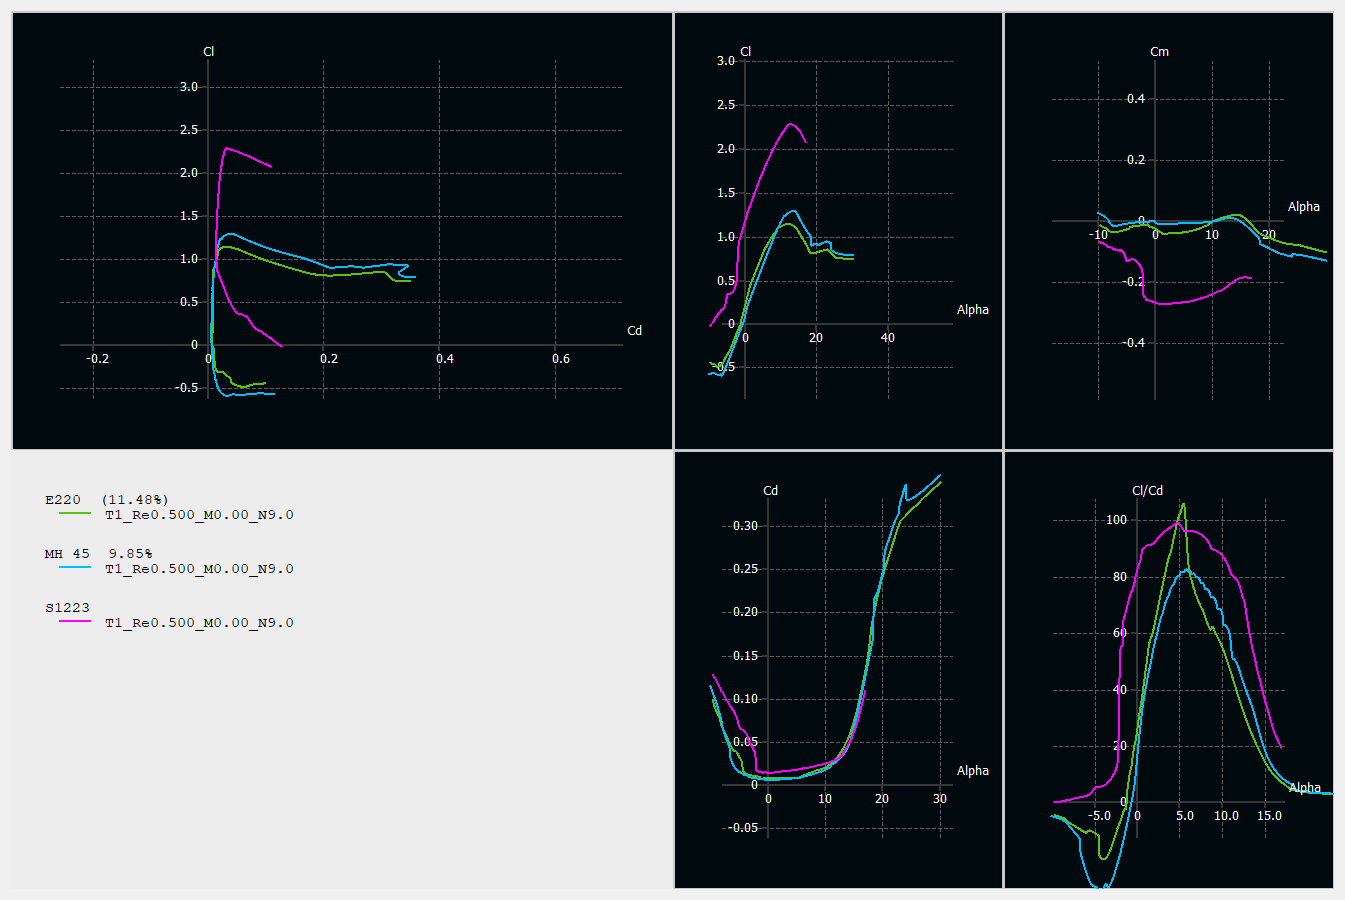
\includegraphics[width=\textwidth]{q2-af-comp.png}
    \end{subfigure}
    \begin{subfigure}[b]{0.45\textwidth}
        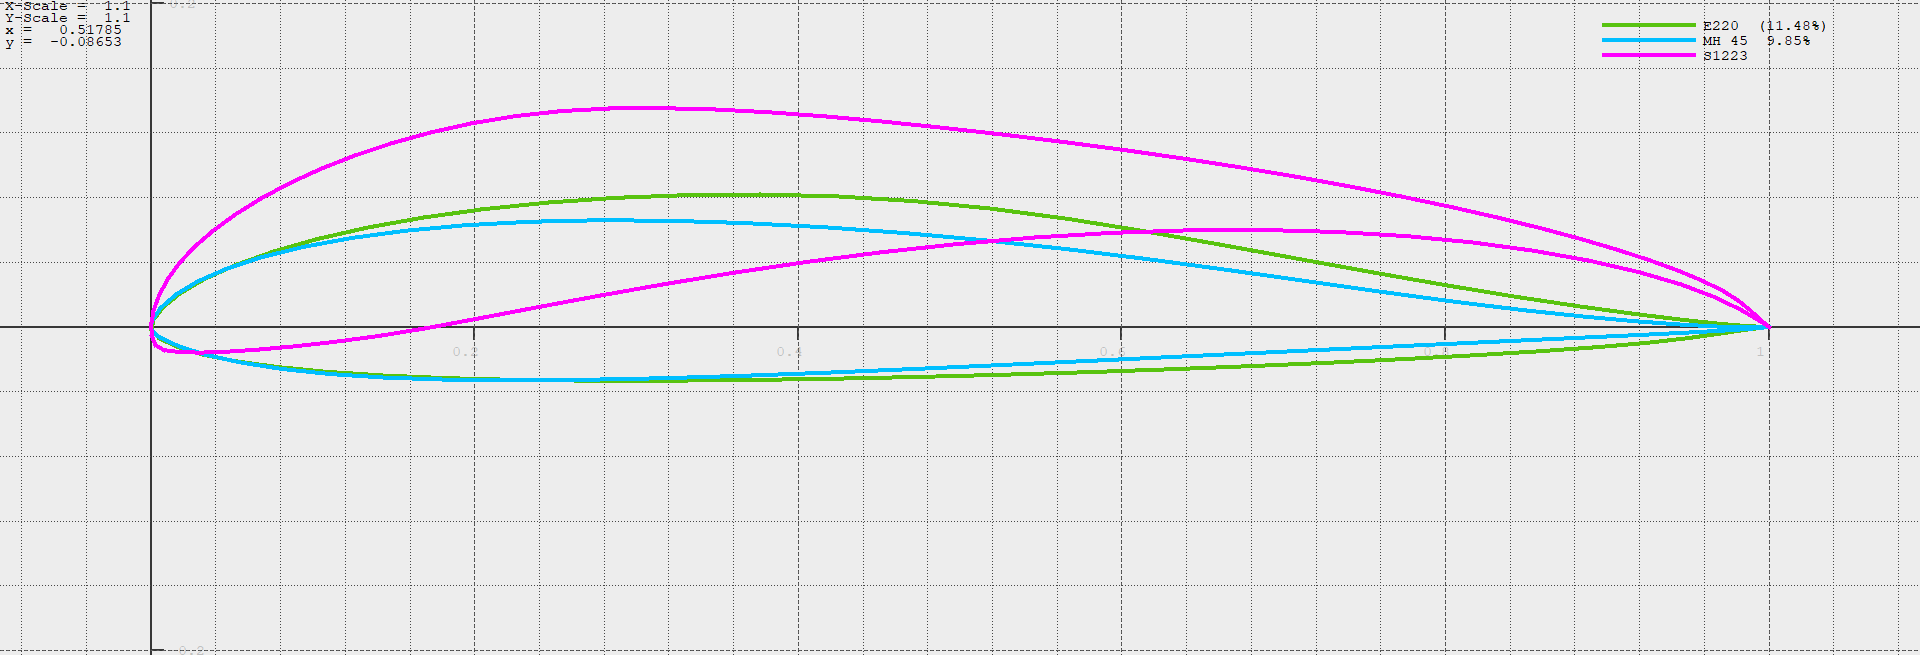
\includegraphics[width=\textwidth]{q2-af-all.png}
    \end{subfigure}
    \caption{Comparing all airfoils}
    \label{fig:q2-af-comp}
\end{figure}
